% !TeX spellcheck = da_DK
\documentclass[../main.tex]{subfiles}


\begin{document}
\lhead{Introduktion}
\chapter{Introduktion}
\section{Problemet og dets perspektiv}
\subsection*{Reinforcement Learning}
%TODO: Tilføj henvisninger til nogle af påstandene
Reinforcement Learning er en af de mest generelle læringsparadigmer i maskinlæring: 
Den enkle opsætning med en agent, et miljø og maksimering af kumulativ skalar-belønning indfører få antagelser om problemets natur og gør sammenligninger til menneskelig læring og fantasier om kunstig generel intelligens fristende.
Når de helt store fremtidsperspektiver lægges til side, er der ofte praktiske mål som selvkørende biler, produktionsrobotter og andre autonome systemer, som bliver set som Reinforcement Learnings potentiale.
Sådanne fysiske agenter i kontinuerte, dynamiske miljøer falder oplagt ind, når man tænker på Reinforcement Learnings formulering og dets familieforhold til kontrolteori, der har rig tradition for styring af fysiske systemer. 

Det er dog unødvendigt begrænsende at se dette lovende maskinlæringsparadigme som dybt forbundet til det kontinuerte og fysiske: Mængden af praktiske beslutningsproblemer er stor og alsidig og der findes vigtige opgaver med helt andre modelleringsudfordringer end f.eks. bevægelse af et robotlegeme.

Diskret optimering er et dybt og velstuderet felt indenfor anvendt matematik og datalogi med klassiske problemer som \textit{Traveling Salesman}, grundlæggende datastrukturer som grafer og matroider og vigtige ingeniørpraktiske anvendelser som operationsanalyse, computationel kemi og planlægningssystemer. 
Disse problemer, der kan udmynte sig i kombinatorisk optimering vha. heltalsprogrammering eller optimering under bibetingelser, har ofte dybe strukturer beskrevet af abstrakt algebra, herunder gruppeteori.
 
I denne rapport vil Reinforcement Learnings generaliserbarhed undersøges ved at bruge det som løsningsmetode til et sådant ikke-trivielt diskret problem, der konventionelt løses med algoritmer fra gruppeteorien.
Det større mål er altså at opnå erfaringer ved at bruge Reinforcement Learning på det kombinatoriske beslutningsproblem, perspektivere det til domænespecifikke løsningsstragier og undersøge udfordringerne med Reinforcement Learning i et stort udfaldsrum. 

\subsection*{Rubiks Terning}

Rubiks terning er et lille, kombinatorisk legetøj opfundet af den ungarske billedhugger og professor i arkitektur Ernö Rubik i 1974. Med 350 mio. solgte terninger regnes den seksfarvede terning som det bedst sælgende legetøj og har fortsat en dedikeret fanskare organiseret i \textit{World Cube Association}, der afholder \textit{speedcuber}-arrangementer og deler praktiske løsningsalgoritmer \cite{RubiksWiki}. 
\begin{figure}[H]
	\centering 
	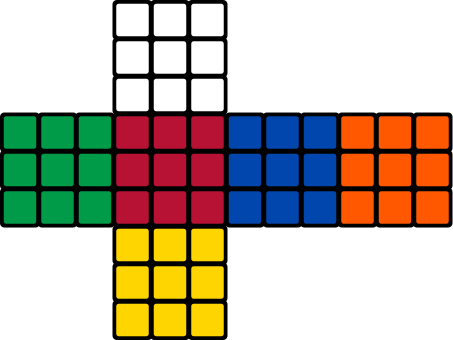
\includegraphics[width=.5\linewidth]{wiki_rubiks_colors}
	\caption{Illustration of de seks farvede sider i en 3x3 Rubiks terning.\protect\footnotemark}
\end{figure}
\footnotetext{Billede: Wikimedia Commons på \url{https://en.wikipedia.org/wiki/File:Rubik\%27s_cube_colors.svg}}
\noindent Målet er at få alle siderne til at være ens som på billedet. 
Har man selv sat sig ned med en sådan terning, virkede problemet måske meget enkelt til at starte med, men man opdager hurtigt, at det er overraskende svært.
Dette skyldes, at der kun er én måltilstand og et utroligt stort tilstandsrum (mere om det senere).
Uden en algoritme vil det formentlig tage et gennemsnitligt menneske utroligt lang tid at finde en måde at løse Rubiks terning på (det tog Rubik selv en måned at finde en løsningsalgoritme til problemet). 
Mennesker kan spille i en time uden at lære særligt meget, men en maskine kan spille mange tusinder af spil og lære på samme måde som et menneske men på meget kortere tid. 



\section{Nyeste litteratur}
\cite{RubiksMedium}
Siden Erno Rubik opfandt sin berømte terning i 1974, er der blevet opfundet adskillige løsningsalgoritmer.
Disse kan overordnet set inddeles i to grupper:
Gruppeteoribaserede algoritmer, fx Kociembas algoritme, og brute force-algoritmer med udgangspunkt i skræddersyede heurestikker.
De forskellige algoritmer har forskellige fordele og ulemper;
nogle skal være lette for mennesker at løse, mens andre er designet til såkaldte speed cubers, der skal løse terningen med så få træk som muligt;
nogle er optimerede til lavt hukommelsesforbrug og andre til at kunne løses hurtigt af computere. 

En ny tilgang til løsningsalgoritmer og diskrete problemer generelt er dyb reinforcement learning.
Et forskerhold fra University of California Irvine har de sidste år gjort store fremskridt med netop denne fremgangsmåde som beskrevet i \textit{Solving the Rubik's Cube Without Human Knowledge} (maj 2018) \cite{HumansBeGone} og senest \textit{Solving the Rubik’s cube with deep reinforcement learning and search} (juli 2019) \cite{SolvingNature}.

DeepCube, der introduceres i \cite{HumansBeGone}, er et dybt neuralt netværk, der bruges som heurestik til at styre en Monte Carlo-træafsøgning, så den kombinatoriske eksplosion undgås.
DeepCube trænes med en approximate policy iteration-algoritme, som forskerne betegner autodidaktisk iteration.
I den løsningsgrafen fra træafsøgningen anvendes breadth first search (BFS) til at finde den korteste løsning.
Metoden formår at løse samtlige tilfældige testtilstande med en medianløsningslængde på 30 træk, hvilket er mindre end eller svarende til løsningsalgoritmer, der er baserede på domæneviden.

DeepCubeA \cite{SolvingNature} kombinerer dyb læring med approksimativ værdiiteration og \emph{batch}-vægtet A*-afsøgning.
Netværket ser kun ét skridt fremad, fordi at se flere skridt fremad eller anvende Monte Carlo-træafsøgning (MCTS) ikke blev fundet til at være bedre.
DeepCubeA bygger på en anden implementation baseret på policy og MCTS.
Den lærte kostfunktion bruges derefter som en heuristik til at finde vejen til løsningstilstanden ved brug af vægtet A*-afsøgning.
DeepCubeA formår at løse alle testkonfigurationer og generaliserer til andre diskrete spil.


\section{Rapportens mål}
Motiveret af Rubiks terning som et miljø for eksperimentation i Reinforcement Learning på svære, kombinatoriske problemer, er det denne rapports mål at udforske mulighederne og begrænsningerne ved at bruge Reinforcement Learning på at løse Rubiks terning.
Der ønskes altså at skabes en løsningsalgoritme, som ikke bruger problem-specifik viden og derfor selv skal lære problemet at kende og udvikle strategier gennem et Reinforcement Learning-paradigme. 
Den generelle form til agenten er på baggrund af litteratursammenligningen valgt til at være en grafsøgende agent, der bruger lærte, dybe neurale netværk som heuristik til at afsøge tilstandsrummet frem til løsningen. For at tage udgangspunkt i en forholdsvis direkte løsningsmetode, det et hovedmål for rapporten at genskabe metoderne (men ikke nødvendigvis resultaterne) for agenten \textit{DeepCube} fra \cite{HumansBeGone}.

Der vil derfor implementeres et dybt neuralt neværk, der både approksimerer en værdi til hver tilstand og den optimale politik hertil. Dette netværk trænes ved brug af en værdiapproksimativ metode kaldet audodidaktisk iteration, der bruger en tidligere version af netværket samt en breddeførst søgning på dybde 1 til at approksimere værdi og politik til hver tilstand.
Når netværket er færdigtrænet, bruges dette til at gennemføre Monte Carlo træsøgning frem til den færdige tilstand. 

I implementationen af en sådan agent er der en del store udfordringer for konvergens som skyldes problemets kombinatoriske eksplosion, der beskrives i \ref{sec:grouptheory}, hvilket gør det til et fokus for rapporten at optimere forudsætninger for læring og sammenligne detaljer i læringsparadigmer.


Konkret er målet med rapporten er at svare på følgende spørgsmål:
\begin{itemize}
	\item Hvor god kan en Reinforcement Learning-algoritme blive til at løse Rubiks terning uden at have adgang til menneskelige heuristikker? Med \textit{god} menes antallet af træk væk fra den løste tilstand, som algoritmen fast kan løse.
	\item Hvilke forhold er optimale i forhold til en stabil konvergens af værdifunktionen, det neurale netværk, i autodidaktisk iteration? Her tænkes på datarepræsentationen og design af træningsproceduren.
	\item Hvor tidseffektiv kan løsning og træning af RL i et problem med så stort udfaldsrum være? Her er både fokus på  at lære den bedst mulige værdi-approkismation, så løsningstid minimeres, men også på at softwaredesign i træningsfasen gør det muligt for agenten at udforske så meget som muligt af udfaldsrummet indenfor overskuelig tid.
\end{itemize}
\noindent
I følgende kapitel \eqref{chp:data} vil datagrundlaget for opgaven blive beskrevet ved først at motivere problemets sværhedsgrad, indføre terminilogi og notation samt vise tilstandsrummets størrelse ved brug af den gruppeteoretiske beskrivelse af terningen. Derefter vil den brugte datastruktur for terningen indføres og afbalancering mellem computationel effektivitet og semantisk passende repræsentation diskuteres.

I kapitel \ref{chp:methods} vil metoderne for løsningen introduceres. Terningemiljøet gennemgås efterfulgt af en introduktion af Reinforcement Learning-opsætningen for problemet. Så introduceres værdi- og politiknetværket samt træningsproceduren, autodidaktisk iteration, samt kostfunktion og optimering for dette. Beskrivelse af løsningsagenten vil så afsluttes med introduktion af Monte Carlo-træsøgningsalgoritmen. Afslutningsvist  vil de gennemførte eksperimenter blive ridset op.



 
\end{document}






















